\documentclass{article}
\usepackage{amsmath}
\usepackage{tikz}
\usetikzlibrary{calc,decorations.markings,decorations.pathmorphing,arrows.meta}
% set up externalization
\usetikzlibrary{external}
\tikzset{external/system call={latex \tikzexternalcheckshellescape -halt-on-error
-interaction=batchmode -jobname "\image" "\texsource";
dvips -o "\image".ps "\image".dvi;
ps2eps "\image.ps"}}
\tikzexternalize
\begin{document}
%---------------------------------------------------------------------------------
%
%\input{./contour_integral_paths/contour_keyhole.tex}
%
%\input{./contour_integral_paths/contour_upper_bc.tex}
%
%\input{./contour_integral_paths/contour_dog-bone_center.tex}
%
%\input{./contour_integral_paths/contour_dog-bone_right.tex}
%
%\input{./contour_integral_paths/contour_upper.tex}
%
%\input{./contour_integral_paths/contour_lower.tex}
%
%\input{./contour_integral_paths/contour_upper_poles.tex}
%
%\input{./contour_integral_paths/contour_2pi_3.tex}
%
%\input{./contour_integral_paths/contour_4pi_3.tex}
%
%\input{./contour_integral_paths/contour_pi_4.tex}
%
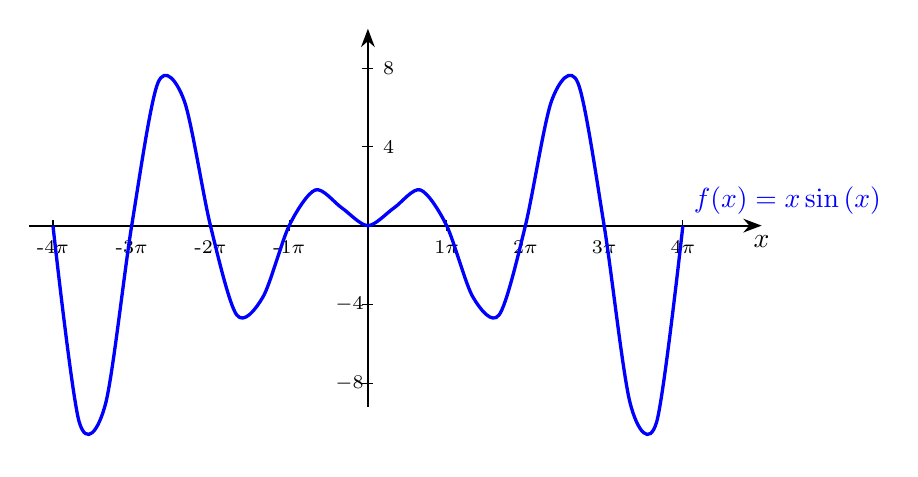
\begin{tikzpicture}[scale=1.0]
  % Configurable parameters
  \def\pie{3.14159265359}
  \newcommand{\axlables}{\normalsize}
  \newcommand{\annotations}{\scriptsize}
  %
  % Axes
  \draw[thick,-Stealth] (-4.3,0) -- (5,0)
    node[below] {\axlables$x$};
  \draw[thick,-Stealth] (0,-2.3) -- (0,2.5);
  % Tick labels
  \foreach \x in {-4,-3,-2,-1,1,2,3,4}
  \draw (\x,2pt)--(\x,-2pt) node[below] {\annotations \x$\pi$};
  % 
  \draw (-2pt,-2) -- (2pt,-2)  node[left]  {\annotations$-8$};
  \draw (-2pt,-1) -- (2pt,-1)  node[left]  {\annotations$-4$};
  \draw (-2pt,1)  -- (2pt,1)   node[right]  {\annotations$4$};
  \draw (-2pt,2)  -- (2pt,2)   node[right]  {\annotations$8$};
  %
  % Plots
  \draw[color=blue,smooth,domain=-4:4,very thick] plot (\x,{\x*\pie/4*sin(\x*\pie r)}) node[above right] {\axlables$f(x) = x \sin{(x)}$};
\end{tikzpicture}
%
%---------------------------------------------------------------------------------
\end{document}